\documentclass[Main]{subfiles}
\begin{document}

\chapter{Data to record}
The system must record the data described in this chapter. The user can create, view, and change the data through the tasks described in Chapter \ref{cha:C}. 
In many cases data has to be exchanged with external systems as specified in Chapter \ref{cha:F}.

Figure \ref{fig:Datamodel} is a data model that gives an overview of the data. 
Each box is a class of data. 
Imagine a pile of file cards behind the box. 
The box symbolizes one of the cards. 

There are relationships between the boxes, shown as crow's feet. 
A crow's foot shows that a card relates to one or many cards in another pile. 
As an example, a group can contain many students, but a student can one relate to only one group. 
Data need not be structured this way in the system, but it must be handled in some way. 

The dotted boxes show data that are (partly) shared with external systems. 

\begin{figure}[hbtp]
\centering
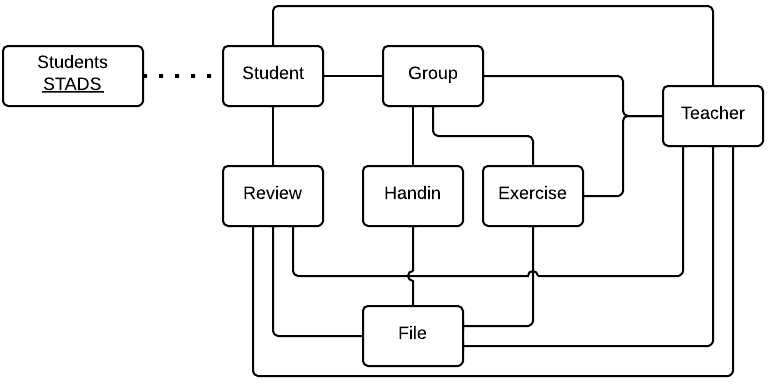
\includegraphics[width=1\textwidth]{DataModel}
\caption{Datamodel}
\label{fig:Datamodel}
\end{figure}

\newpage

\section{Student}
A \textit{Student} is a one of the participants of the course.
\begin{DataIntro}
\rExample{}
\rSource{Students are enrolled at the start of the course. 
Students are imported from STADS.}
\rUse{Students are assigned to a \textit{Group} and can have speciel case regarding handins.}
\end{DataIntro}

\begin{DataTable}
\Record
{ID}
{Each student of the course will be assigned an ID to identify the student.}
{}


\Record
{Student number. 
\\
Copied from the STADS database. 
This will serve as a static reference for updates later on.}
{Each student have a personal number assigned by the university to identify them}
{}

\Record
{Full name\\
Copied from the STADS database.}
{This will be shown along with a student's handin and review.}
{}

\Record
{Password}
{Along with the student number this will serve as a login to the system.}
{}


\Record
{Email address\\
Imported from the STADS database.}
{When a notification is ready for a student it can be send to this email}
{}
\end{DataTable}





\newpage

\section{Group}
A \textit{Group} is a list of students who will deliver handins together.
\begin{DataIntro}
\rExample{}
\rSource{Have a minimum size of 1 student.}
\rUse{Groups deliver handins.
A group can be of only 1 student should this student choose to deliver a handin on his/her own.
Each student can only be assigned to one group pr. course.}
\end{DataIntro}

\begin{DataTable}

\Record
{ID\\
Each group will have an ID to serve as reference to the handins.}
{}
{}

\Record
{Name\\
Autogenerated}
{Will be shown for the teacher on reviews.}
{}


\Record
{List of studens.\\
Each student of the group shall be listed here}
{A list contains 3 students, reference by ID.}
{}


\end{DataTable}




\newpage

\section{Teacher}
A \textit{Teacher} is a lecturer of the course.

\begin{DataIntro}
\rExample{}
\rSource{There will be at least 1 teacher at a course.}
\rUse{Teachers upload exercises and deadline.\\
Teachers approve reviews.}
\end{DataIntro}

\begin{DataTable}

\Record
{ID\\
Each teacher will have an ID to serve as reference for uploading exercises.}
{}
{}

\Record
{Full name}
{Name of the teacher will be shown on exercises and notifications for students.}
{}

\end{DataTable}



\newpage

\section{Exercise}
An \textit{Exercise} is a a description for a \textit{Handin}.
\begin{DataIntro}
\rExample{}
\rSource{Created by a \textit{Teacher}.}
\rUse{\textit{Students} most solve the exercises within the provided deadline in groups.}
\end{DataIntro}

\begin{DataTable}

\Record
{ID\\
Each exercise has a unique ID.}
{}
{}

\Record
{Name}
{Each exercise has a name to be displayed for the students.}
{}

\Record
{Deadline.}
{A date the students must deliver handins before.}
{}


\Record
{File(s)}
{An exercise can contain one or more files}
{}


\Record
{Commentary}
{An exercise can have a comment on it}
{}


\Record
{Timestamp\\}
{A date for when uploaded}
{}
\end{DataTable}

\fxnote{2 uploads giver forskellige filer, men samme navn}





\newpage

\section{Handin}

	
\begin{DataIntro}
\rExample{}
\rSource{Student upload handins\fxnote{There can be multiple upload before a deadline}}
\rUse{Handins will be assigned to review for other students}
\end{DataIntro}

\begin{DataTable}

\Record
{ID\\
Used to track a specific assignment}
{}
{}

\Record
{GroupID}
{ID for the group who delivered it.}
{}


\Record
{Timestamp}
{Timestamp for the upload.}
{}
\end{DataTable}


\newpage

\section{Review}
Reviews are made by a single student for another student's handin. 
The review can be uploaded multiple time in different versions -- only the last will be shown to the other student.

\begin{DataIntro}
\rExample{}
\rSource{Student.}
\rUse{The reviews include notes for improvement for the other student.}
\end{DataIntro}

\begin{DataTable}

\Record
{ID\\
A unique ID to keep track of a review submission.}
{}
{}


\Record
{Student ID}
{Reviewer's student ID to trace who reviews the handin.}
{}


\Record
{Timestamp}
{Used to track when the review has been uploaded.}
{}


\Record
{Files}
{Optional -- contains comments for the handin.}
{}


\Record
{Comments}
{Optional\fxnote{Only if no file has been uploaded} -- contains comment for the handin.}
{}


\Record
{Ready for deliver}
{Field must be checked to deliver a review, should one change mind after a review.
This must be checked before the deadline.}
{}
\end{DataTable}




\newpage

\section{Files}
Files will be multiple versions of exercises, handins and reviews.
All versions must be saved and possible to retrieve.

\begin{DataIntro}
\rExample{•}
\rSource{Uploads as exercises, handins or reviews.}
\rUse{These files can be downloaded and uploaded by students for when submitting handins, when viewing an exercise, submitting reviews and looking at reviews of own handins.}
\end{DataIntro}

\begin{DataTable}

\Record
{ID}
{Unique identifier for system retrieval and storage.}
{}


\Record
{Name}
{The name of the file}
{}


\Record
{Binary storage}
{Storage of the file can be done in binary form}
{}
\end{DataTable}





\end{document}